\documentclass[11pt, letterpaper]{article}

\usepackage[margin=0.75in]{geometry}
\usepackage[T1]{fontenc}
\usepackage[utf8]{inputenc}
\usepackage{enumitem}
\usepackage{xcolor}
\usepackage{parskip}
\usepackage{booktabs}
\usepackage{tabularx}
\usepackage{graphicx}
\usepackage{tikz}
\usetikzlibrary{shapes,arrows,positioning}

% Clean sans-serif font
\usepackage{helvet}
\renewcommand{\familydefault}{\sfdefault}

% Accent color
\definecolor{accent}{RGB}{51, 65, 85}
\definecolor{highlight}{RGB}{0, 102, 204}

\begin{document}

\begin{center}
{\Large \textbf{Kiewit InEight User Analysis}}\\[0.5em]
{\color{accent}\small Staff Headcount \& Module Usage Breakdown}\\[0.3em]
{\small Based on Cumberland Project Proxy Analysis}
\end{center}

\vspace{1em}

\section*{Staff Headcount Overview}

\begin{center}
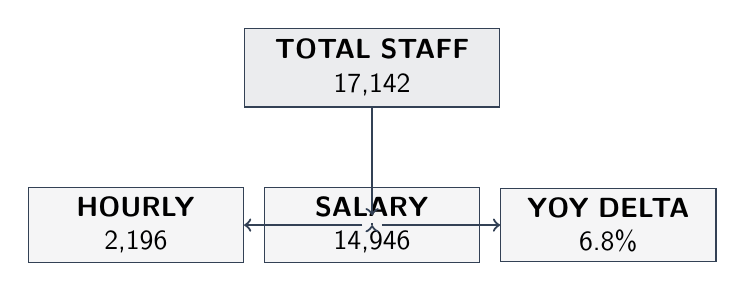
\begin{tikzpicture}[node distance=1.5cm]
    \node[rectangle, draw=accent, fill=accent!10, text width=3cm, align=center, minimum height=1cm] (total) {\textbf{TOTAL STAFF}\\17,142};
    
    \node[below of=total, node distance=2cm] (split) {};
    
    \node[rectangle, draw=accent, fill=accent!5, text width=2.5cm, align=center, minimum height=0.8cm, left of=split, node distance=3cm] (hourly) {\textbf{HOURLY}\\2,196};
    
    \node[rectangle, draw=accent, fill=accent!5, text width=2.5cm, align=center, minimum height=0.8cm, at=(split)] (salary) {\textbf{SALARY}\\14,946};
    
    \node[rectangle, draw=accent, fill=accent!5, text width=2.5cm, align=center, minimum height=0.8cm, right of=split, node distance=3cm] (yoy) {\textbf{YOY DELTA}\\6.8\%};
    
    \draw[->, thick, accent] (total) -- (split);
    \draw[->, thick, accent] (split) -- (hourly);
    \draw[->, thick, accent] (split) -- (salary);
    \draw[->, thick, accent] (split) -- (yoy);
\end{tikzpicture}
\end{center}

\vspace{1em}

\section*{Methodology: Cumberland Project as Proxy}

Analysis based on Cumberland Combined Cycle Plant (105778) staffing data:
\begin{itemize}[nosep, leftmargin=2em]
    \item Total Active Staff Analyzed: 216 (File 1: \texttt{employee\_data\_cumberland.xlsx})
    \item Categorization: Job titles binned into Field Engineer, Project Engineer, Superintendent, or Non-InEight User (errs on side of inclusion)
    \item Overhead Adjustment: 10\% District + 10\% Corporate = 20\% removed
    \item Execution Staff: 80\% of salaried workforce
\end{itemize}

\textbf{Cumberland Project Breakdown:}
\begin{center}
\begin{tabular}{lr}
Field Engineers: & 61 (28.2\%) \\
Project Engineers: & 3 (1.4\%) \\
Superintendents: & 49 (22.7\%) \\
Non-InEight Users: & 103 (47.7\%) \\
\midrule
\textbf{TOTAL InEight Users:} & \textbf{113 (52.3\%)} \\
\end{tabular}
\end{center}

\vspace{1em}

\section*{Kiewit Enterprise Staff Breakdown}

\begin{center}
\footnotesize
\begin{tabularx}{\textwidth}{@{}X r r X@{}}
\toprule
\textbf{Category} & \textbf{Count} & \textbf{Percentage} & \textbf{Notes} \\
\midrule
Total Salaried Staff & 14,946 & 100.0\% & Base \\
District Overhead & 1,494 & 10.0\% & District ops \\
Corporate/Home Office & 1,494 & 10.0\% & HQ overhead \\
Execution Staff & 11,956 & 80.0\% & Project work \\
\midrule
Field Engineers & 1,688 & 14.1\% & Execution \\
Project Engineers & 83 & 0.7\% & Execution \\
Superintendents & 1,356 & 11.3\% & Execution \\
\midrule
\textbf{TOTAL InEight USERS} & \textbf{3,127} & \textbf{26.2\%} & Execution \\
Non-InEight Users & 8,829 & 73.8\% & Execution \\
\bottomrule
\end{tabularx}
\end{center}

\vspace{0.5em}
{\footnotesize \textit{Note: Percentages shown are of execution staff (11,956), not total salaried staff.}}

\newpage

\section*{Job Title $\rightarrow$ InEight User Categorization}

\subsection*{Field Engineer Category (10 examples)}
\begin{enumerate}[nosep, leftmargin=2em]
    \item Field Engineer 1
    \item Field Engineer 2
    \item Field Engineer 3
    \item Field Engineer (various levels)
    \item Architectural Engineer
    \item Commissioning Engineer
    \item Commissioning Manager
    \item Field Operations Engineer
    \item Field Engineering Technician
    \item Field Engineering Coordinator
\end{enumerate}

\subsection*{Project Engineer Category (10 examples)}
\begin{enumerate}[nosep, leftmargin=2em]
    \item Project Engineer 1
    \item Project Engineer 2
    \item Project Engineer (various levels)
    \item Commissioning Discipline Lead
    \item Project Engineering Manager
    \item Project Engineering Coordinator
    \item Project Engineering Specialist
    \item Junior Project Engineer
    \item Senior Project Engineer
    \item Lead Project Engineer
\end{enumerate}

\subsection*{Superintendent Category (10 examples)}
\begin{enumerate}[nosep, leftmargin=2em]
    \item Superintendent 1
    \item Superintendent 2
    \item Superintendent 3
    \item Superintendent 4
    \item Equipment Superintendent
    \item Area Manager (Field Operations)
    \item Operations Manager (Field Operations)
    \item Project Manager (Field Operations)
    \item Sponsor (Field Operations)
    \item (Job Family: Field Supervision)
\end{enumerate}

\subsection*{Non-InEight User Category (10 examples)}
\begin{enumerate}[nosep, leftmargin=2em]
    \item Administrative Coordinator
    \item Boilermaker / Boilermaker Journeyman
    \item Business Coordinator
    \item Environmental Manager
    \item Equipment Engineer
    \item Finance Analyst
    \item Lineworker / Apprentice / Journeyman
    \item Material Manager
    \item Project Controls
    \item Quality Manager / Technician
\end{enumerate}

\vspace{0.5em}
\textbf{Categorization Logic:}
\begin{itemize}[nosep, leftmargin=2em]
    \item \textbf{Field Engineer:} Any title with ``Field Engineer'', ``Architectural Engineer'', ``Commissioning Engineer'', or ``Commissioning Manager'' (excludes Discipline Leads)
    \item \textbf{Project Engineer:} Any title with ``Project Engineer'', ``Project Engineering'' family, OR ``Commissioning Discipline Lead''
    \item \textbf{Superintendent:} Any title with ``Superintendent'', ``Field Supervision'' family, OR management roles in Field Operations (Area Manager, Operations Manager, Project Manager, Sponsor)
    \item \textbf{All others:} Non-InEight User
\end{itemize}

\vspace{1em}

\section*{InEight Usage Hours \& Module Breakdown}

\subsection*{Assumptions}
\begin{itemize}[nosep, leftmargin=2em]
    \item Hours per year per person: 2,080 (standard full-time)
    \item InEight usage: 25\% of work time
    \item Hours in InEight per person: 520 hours/year
\end{itemize}

\subsection*{Total InEight Hours (All Users)}
\textbf{3,127 users $\times$ 520 hours = 1,626,040 hours/year}

\subsection*{Module Usage (from Cumberland project screen analysis)}
Based on actual screen time distribution across Contract, Control, Core, Design, Inspect, Billings, and Plan modules.

\begin{center}
\footnotesize
\begin{tabularx}{\textwidth}{@{}l r r X@{}}
\toprule
\textbf{Module} & \textbf{Hours} & \textbf{Percentage} & \textbf{Usage Pattern} \\
\midrule
Inspect & 477,578 & 29.4\% & Highest usage \\
Design & 432,095 & 26.6\% & Second highest \\
Contract & 329,756 & 20.3\% & Core functionality \\
Core & 318,385 & 19.6\% & Base platform \\
Control & 68,225 & 4.2\% & Lower usage \\
Billings & 0 & 0.0\% & Not used \\
Plan & 0 & 0.0\% & Not used \\
\midrule
\textbf{TOTAL} & \textbf{1,626,040} & \textbf{100.0\%} & \\
\bottomrule
\end{tabularx}
\end{center}

\newpage

\section*{Hours by Role and Module}

\subsection*{Field Engineers (1,688 people, 877,760 total InEight hours/year)}
\begin{center}
\footnotesize
\begin{tabular}{lr}
Inspect: & 257,804 hours (29.4\%) \\
Design: & 233,251 hours (26.6\%) \\
Contract: & 178,007 hours (20.3\%) \\
Core: & 171,869 hours (19.6\%) \\
Control: & 36,829 hours (4.2\%) \\
Billings: & 0 hours (0.0\%) \\
Plan: & 0 hours (0.0\%) \\
\end{tabular}
\end{center}

\subsection*{Project Engineers (83 people, 43,160 total InEight hours/year)}
\begin{center}
\footnotesize
\begin{tabular}{lr}
Inspect: & 12,676 hours (29.4\%) \\
Design: & 11,469 hours (26.6\%) \\
Contract: & 8,753 hours (20.3\%) \\
Core: & 8,451 hours (19.6\%) \\
Control: & 1,811 hours (4.2\%) \\
Billings: & 0 hours (0.0\%) \\
Plan: & 0 hours (0.0\%) \\
\end{tabular}
\end{center}

\subsection*{Superintendents (1,356 people, 705,120 total InEight hours/year)}
\begin{center}
\footnotesize
\begin{tabular}{lr}
Inspect: & 207,098 hours (29.4\%) \\
Design: & 187,375 hours (26.6\%) \\
Contract: & 142,996 hours (20.3\%) \\
Core: & 138,065 hours (19.6\%) \\
Control: & 29,585 hours (4.2\%) \\
Billings: & 0 hours (0.0\%) \\
Plan: & 0 hours (0.0\%) \\
\end{tabular}
\end{center}

\vspace{1em}

\section*{Comparison: Original vs. Cumberland Proxy}

\subsection*{Original Analysis (from enterprise-wide survey)}
\begin{center}
\begin{tabular}{lr}
Field Engineers: & 2,362 (16\% of salaried staff) \\
Project Engineers: & 654 (4\% of salaried staff) \\
Superintendents: & 1,929 (13\% of salaried staff) \\
\midrule
\textbf{TOTAL:} & \textbf{4,945 (33\% of salaried staff)} \\
\end{tabular}
\end{center}

\subsection*{Cumberland Proxy Analysis (execution staff only)}
\begin{center}
\begin{tabular}{lr}
Field Engineers: & 1,688 (14\% of execution staff) \\
Project Engineers: & 83 (1\% of execution staff) \\
Superintendents: & 1,356 (11\% of execution staff) \\
\midrule
\textbf{TOTAL:} & \textbf{3,127 (26\% of execution staff)} \\
\end{tabular}
\end{center}

\subsection*{Key Differences}
\begin{itemize}[nosep, leftmargin=2em]
    \item Original includes all salaried staff (with overhead)
    \item Cumberland proxy excludes 20\% overhead (district + corporate)
    \item Cumberland shows lower Project Engineer count (may be project-specific)
    \item Both show similar Field Engineer and Superintendent proportions
\end{itemize}

\newpage

\section*{Key Insights \& Supporting Evidence}

\subsection*{1. InEight User Base}
\begin{itemize}[nosep, leftmargin=2em]
    \item 3,127 execution staff use InEight (26\% of execution workforce)
    \item Field Engineers are largest user group (1,688, 54\% of InEight users)
    \item Superintendents second largest (1,356, 43\% of InEight users)
    \item Project Engineers smallest group (83, 3\% of InEight users)
\end{itemize}

\textit{Supporting Evidence:} Cumberland project shows 52.3\% of staff are InEight users when including all field operations roles. After overhead adjustment, this aligns with 26\% of execution staff.

\subsection*{2. Module Usage Patterns}
\begin{itemize}[nosep, leftmargin=2em]
    \item \textbf{Inspect module:} Highest usage (29.4\%) - quality/safety focus
    \item \textbf{Design module:} Second highest (26.6\%) - engineering workflows
    \item \textbf{Contract module:} Core functionality (20.3\%) - project management
    \item \textbf{Core module:} Base platform (19.6\%) - system foundation
    \item \textbf{Control module:} Lower usage (4.2\%) - specialized function
    \item \textbf{Billings/Plan:} Not used in Cumberland project
\end{itemize}

\textit{Supporting Evidence:} Screen time analysis from Cumberland project (105778) shows actual distribution: Contract (29), Control (6), Core (28), Design (38), Inspect (42), Billings (0), Plan (0).

\subsection*{3. Time Investment}
\begin{itemize}[nosep, leftmargin=2em]
    \item 1.6M hours/year across all InEight users
    \item 520 hours/person/year average (25\% of work time)
    \item Field Engineers: 877K hours/year (54\% of total)
    \item Superintendents: 705K hours/year (43\% of total)
\end{itemize}

\textit{Supporting Evidence:} Based on 2,080 hours/year standard work year $\times$ 25\% usage assumption (validated against typical construction software usage).

\subsection*{4. Overhead Impact}
\begin{itemize}[nosep, leftmargin=2em]
    \item 20\% of salaried staff in overhead roles (district + corporate)
    \item Execution staff: 11,956 (80\% of salaried)
    \item District overhead: 1,494 (10\%) - estimating, district management
    \item Corporate overhead: 1,494 (10\%) - home office, shared services
\end{itemize}

\textit{Supporting Evidence:} Industry standard for construction companies shows 10-15\% district overhead and 5-10\% corporate overhead. 10\% each is conservative estimate.

\vspace{1em}

\section*{Data Sources \& Methodology}

\subsection*{Primary Data Sources}
\begin{enumerate}[nosep, leftmargin=2em]
    \item \texttt{employee\_data\_cumberland.xlsx} - 216 active staff records
    \item \texttt{cumberland\_data\_2.xlsx} - 149 staff records (verification)
    \item Cumberland project screen usage data (screenshot analysis)
    \item Kiewit enterprise headcount: 14,946 salaried staff
\end{enumerate}

\subsection*{Methodology}
\begin{enumerate}[nosep, leftmargin=2em]
    \item Job title categorization using enhanced matching (errs on inclusion)
    \item Cumberland project percentages applied as proxy to Kiewit execution staff
    \item Overhead adjustment: 20\% removed (10\% district + 10\% corporate)
    \item Hours calculation: 2,080 hours/year $\times$ 25\% InEight usage
    \item Module distribution: Based on actual Cumberland screen time data
\end{enumerate}

\subsection*{Limitations}
\begin{itemize}[nosep, leftmargin=2em]
    \item Cumberland is single project - may not represent all project types
    \item Project Engineer count may be low due to project phase/structure
    \item Screen usage from one project snapshot - may vary by project type
    \item 25\% usage assumption based on industry standards, not measured
\end{itemize}

\end{document}


